\documentclass[10pt]{book}

%These tell TeX which packages to use.
\usepackage{array,epsfig}
\usepackage{amsmath}
\usepackage{amsfonts}
\usepackage{amssymb}
\usepackage{amsxtra}
\usepackage{amsthm}
\usepackage{mathrsfs}
\usepackage{color}
\usepackage{enumitem}
%\usepackage{mdframed}
\usepackage[most]{tcolorbox}
\usepackage{pgfplots}
\usetikzlibrary{arrows}
\pgfplotsset{compat=1.6}

\pgfplotsset{soldot/.style={color=black,only marks,mark=*}} \pgfplotsset{holdot/.style={color=black,fill=white,only marks,mark=*}}

%Here I define some theorem styles and shortcut commands for symbols I use often
\theoremstyle{definition}
\newtheorem{defn}{Definition}
\newtheorem{thm}{Theorem}
\newtheorem{cor}{Corollary}
\newtheorem*{rmk}{Remark}
\newtheorem{lem}{Lemma}
\newtheorem*{joke}{Joke}
\newtheorem{ex}{Example}
\newtheorem*{soln}{Solution}
\newtheorem{prop}{Proposition}

\newcommand{\lra}{\longrightarrow}
\newcommand{\ra}{\rightarrow}
\newcommand{\surj}{\twoheadrightarrow}
\newcommand{\graph}{\mathrm{graph}}
\newcommand{\bb}[1]{\mathbb{#1}}
\newcommand{\Z}{\bb{Z}}
\newcommand{\Q}{\bb{Q}}
\newcommand{\R}{\bb{R}}
\newcommand{\C}{\bb{C}}
\newcommand{\N}{\bb{N}}
\newcommand{\M}{\mathbf{M}}
\newcommand{\m}{\mathbf{m}}
\newcommand{\MM}{\mathscr{M}}
\newcommand{\HH}{\mathscr{H}}
\newcommand{\Om}{\Omega}
\newcommand{\Ho}{\in\HH(\Om)}
\newcommand{\bd}{\partial}
\newcommand{\del}{\partial}
\newcommand{\bardel}{\overline\partial}
\newcommand{\textdf}[1]{\textbf{\textsf{#1}}\index{#1}}
\newcommand{\img}{\mathrm{img}}
\newcommand{\ip}[2]{\left\langle{#1},{#2}\right\rangle}
\newcommand{\inter}[1]{\mathrm{int}{#1}}
\newcommand{\exter}[1]{\mathrm{ext}{#1}}
\newcommand{\cl}[1]{\mathrm{cl}{#1}}
\newcommand{\ds}{\displaystyle}
\newcommand{\vol}{\mathrm{vol}}
\newcommand{\cnt}{\mathrm{ct}}
\newcommand{\osc}{\mathrm{osc}}
\newcommand{\LL}{\mathbf{L}}
\newcommand{\UU}{\mathbf{U}}
\newcommand{\support}{\mathrm{support}}
\newcommand{\AND}{\;\wedge\;}
\newcommand{\OR}{\;\vee\;}
\newcommand{\Oset}{\varnothing}
\newcommand{\st}{\ni}
\newcommand{\wh}{\widehat}
%Pagination stuff.
\setlength{\topmargin}{-0.75in}
\setlength{\oddsidemargin}{0in}
\setlength{\evensidemargin}{0in}
\setlength{\textheight}{9.in}
\setlength{\textwidth}{6.5in}
\pagestyle{empty}
\begin{document}
\begin{flushleft}
Name:\underline{\hspace{13cm}}Date:\underline{\hspace{2cm}}
\end{flushleft}
\begin{center}
{\Large Math 1041-012 \hspace{0.5cm} Section 4.3}
\end{center}
%\vspace{0.2 cm}

\begin{tcolorbox}
\subsection*{Increasing/Decreasing Test}
Given a function $f(x)$ on an interval...
\begin{itemize}
    \item If \underline{\hspace{3cm}} on an interval, then $f$ is increasing on the interval.
    \item If \underline{\hspace{3cm}} on an interval, then $f$ is decreasing on the interval.
\end{itemize}
\end{tcolorbox}
\subsection*{Visual Example} The graph of $f$ is shown below. State the open intervals where (a) $f(x)$ is increasing and (b) $f(x)$ is decreasing.
\begin{figure}[h!]
    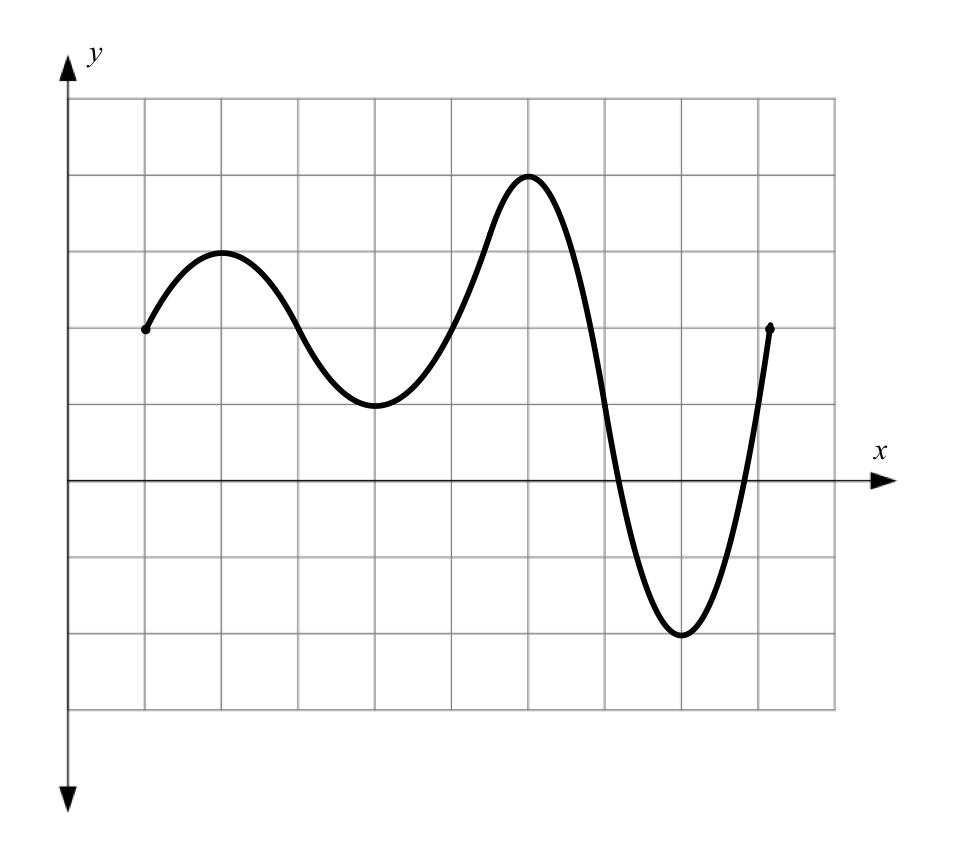
\includegraphics[width=3in]{Rolles1.png}
\end{figure}
\subsection*{Function Example} Find where the function $f(x)=3x^4-4x^3-12x^2+5$ is increasing and where it is decreasing?
\clearpage
\begin{tcolorbox}
\subsection*{First Derivative Test}
Suppose that $c$ is a \underline{\hspace{3cm}} of a continuous function $f$...
\begin{itemize}
    \item If $f'$ changes from \underline{\hspace{1cm}} to \underline{\hspace{1cm}} at $c$, then $f$ has a local maximum at $c$.
    \item If $f'$ changes from \underline{\hspace{1cm}} to \underline{\hspace{1cm}} at $c$, then $f$ has a local minimum at $c$.
    \item If $f'$ has the same sign on either side of $c$, then $f$ has no local max/min at $c$. 
\end{itemize}
\textit{In other words:} A sign change with $f'$ ($f$ continuous) at $c$ means you have a local max/min at $c$.
\end{tcolorbox}
\begin{figure}[h!]
    \centering
    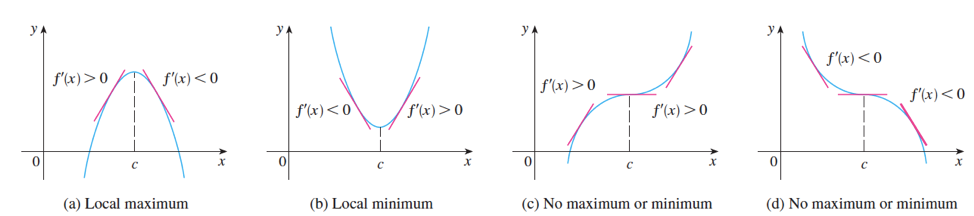
\includegraphics{FirstDTest.png}
\end{figure}
\subsection*{Example 3} State the intervals where $f$ is increasing and decreasing, and find the local minimum and maximum values of the function $f(x)=2x^3-9x^2+12x-3$.
\clearpage
\begin{tcolorbox}
\subsection*{Concavity and Concavity Tests} 
\begin{itemize}
    \item If $f$ lies above all tangents on an interval, then $f$ is \underline{\hspace{3cm}} on the interval. This means \underline{\hspace{2cm}} on the interval.
    \item If $f$ lies below all tangents on an interval, then $f$ is \underline{\hspace{3cm}} on the interval. This means \underline{\hspace{2cm}} on the interval.
    \item A point where $f$ changes concavity is called an \underline{\hspace{4cm}}.
\end{itemize}
\end{tcolorbox}
\subsection*{Visual Example} The graph of $f$ is given below.
\begin{figure}[h!]
    \centering
    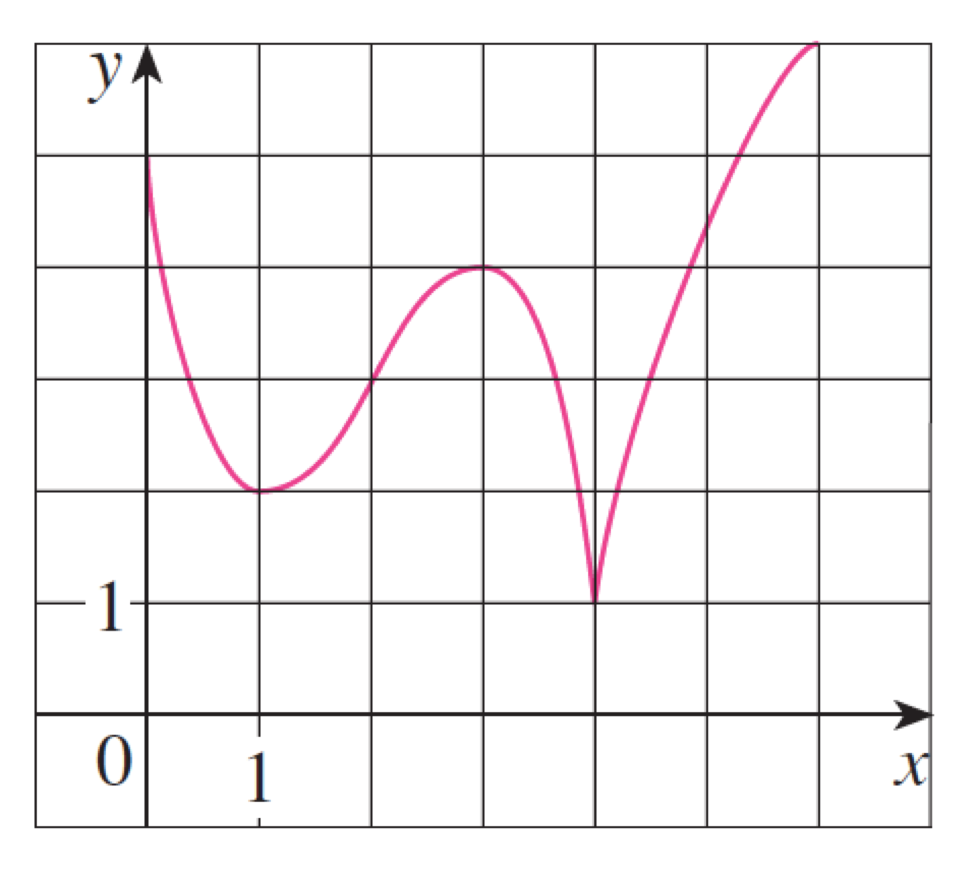
\includegraphics[width=3in]{GraphA.png}
\end{figure}
\begin{enumerate}[label=(\alph*)]
    \item State the open intervals where $f$ is increasing.\vspace{1cm}
    \item State the open intervals where $f'(x)<0$.\vspace{1cm}
    \item State the open intervals where $f''(x)>0$.\vspace{1cm}
    \item State the open intervals where $f$ is concave down.\vspace{1cm}
    \item State the coordinates where there is an inflection point (if any).
\end{enumerate}
\clearpage
\subsection*{Example: Sketching}
Sketch a possible graph of a function $f$ that satisfies the following conditions:
\begin{itemize}
    \item $f'(x)>0$ on $(-\infty,1)$,
    \item $f'(x)<0$ on $(1,\infty)$,
    \item $f''(x)>0$ on $(-\infty,-2), (2,\infty)$,
    \item $f''(x)<0$ on $(-2,2)$,
    \item $\displaystyle\lim_{x\rightarrow-\infty}f(x)=-2$ and $\displaystyle\lim_{x\rightarrow\infty}f(x)=0$\vspace{1cm}
\end{itemize}
\begin{tcolorbox}
\subsection*{Second Derivative Test} Assume $f''$ is continuous near $c$.
\begin{itemize}
    \item If $f'(c)=0$ AND $f''(c)>0$, then $f$ has local minimum at $c$.
    \item If $f'(c)=0$ AND $f''(c)<0$, then $f$ has local minimum at $c$.
\end{itemize}
\textit{In other words:} The concavity at a critical number tells you whether it is local max/min.\\ \\
\textbf{Note:} If $f''(c)=0$, then NO CONCLUSION.
If $f''(c)$ DNE, then NO CONCLUSION. In both cases use the First Derivative test.
\end{tcolorbox}
\subsection*{Example 6} Given $y=x^4-4x^3$, determine the intervals of concavity, local max/min, inflection points. Then use this information to sketch the curve.
\clearpage
\subsection*{Example 7} Sketch the graph of the function $f(x)=x^{2/3}(6-x)^{1/3}$.
\clearpage
\subsection*{Example 8} Use the first and second derivatives of $f(x)=e^{1/x}$, together with asymptotes to sketch its graph.
\end{document}